% this file is called up by thesis.tex
% content in this file will be fed into the main document

\chapter{Design} % top level followed by section, subsection


% ----------------------- paths to graphics ------------------------

% change according to folder and file names
\ifpdf
    \graphicspath{{7/figures/PNG/}{7/figures/PDF/}{7/figures/}}
\else
    \graphicspath{{7/figures/EPS/}{7/figures/}}
\fi


% ----------------------- contents from here ------------------------
% 

\section{Framework}

In this section we describe the tools and techniques used with the OpenCSD
framework, detail modules and functionality and show the external dependencies
as well as internal relationships.

Firstly, OpenCSD consist of many external dependencies, most prominently SPDK
and uBPF. To reduce the barrier to entree and simplify ease of use OpenCSD
installs the majority of external dependencies in a local isolated build
directory. Subsequently, these dependencies are made available through an
environment file which configures variables such as \textit{PATH} and
\textit{LD\_LIBRARY\_PATH}. In addition, OpenCSD offers a QEMU installation and
accompanying qcow image to emulate a ZNS SSDs due to the limited availability of
these SSDs currently. However, the use of QEMU is entirely optional. Finally,
CMake is used to orchestrate the installation of dependencies and binary
targets. Due to limitations it is advised to rerun cmake after each make
command, this prevents unnesecarry recompilation of external dependencies.

As said OpenCSD is comprised of modules using a component architecture.
Aditionally, Each module is compiled as a static or shared library to reduce
coupling. This creates an explicit nature of exchanging information between
linked libraries tgat allows to identify feasability problems at an early stage.
This is opposed to potentially only identifying such issues when creating a
first prototype. A trivial example of such infeasabilities would be using shared
memory mutexes to synchronize filesystem and CSx program behavior.

The overall modules of OpenCSD are shown in figure
\ref{figure:moduledependencies} along with any external or internal
dependencies.

% Diagram with overview of different modules and their used as well as
% relationships. Also show integration of open-source technologies.

\begin{figure}
    \centering
	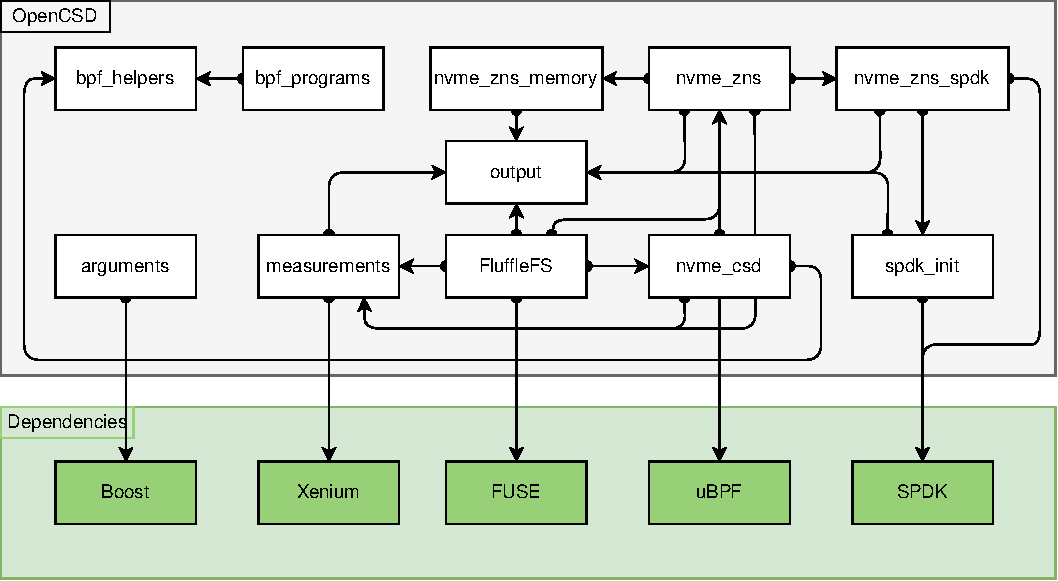
\includegraphics[width=1\textwidth]{resources/images/module-dependencies.pdf}
	\caption{Overview of all OpenCSD components and their depends-on relations}
    % \includesvg[width=0.6\columnwidth]{resources/images/module-dependencies}
    \label{figure:moduledependencies}
\end{figure}

\section{Filesystem}

% Two write pointers, one for RANDOM ZONE and one for LOG ZONE. Use of ZNS is
% optional but allows for lower write-amplification and more explicit garbage
% collection

\subsection{Concurrency}

\section{Offloading}

% Filesystem extended attributes, PID + INODE

\section{Design for Manufacter}

% Describe how the design would change for a real world, practical
% implementation. Take the ICD loader diagram as base.

% ---------------------------------------------------------------------------
% ----------------------- end of thesis sub-document ------------------------
% ---------------------------------------------------------------------------